\documentclass[12pt,letterpaper]{article}
\usepackage[utf8]{inputenc}
\usepackage[spanish]{babel}
\usepackage{graphicx}
\usepackage[left=2cm,right=2cm,top=2cm,bottom=2cm]{geometry}
\usepackage{graphicx} % figuras
% \usepackage{subfigure} % subfiguras
\usepackage{float} % para usar [H]
\usepackage{amsmath}
%\usepackage{txfonts}
\usepackage{stackrel} 
\usepackage{multirow}
\usepackage{enumerate} % enumerados
\renewcommand{\labelitemi}{$-$}
\renewcommand{\labelitemii}{$\cdot$}
% \author{}
% \title{Caratula}
\begin{document}

% Fancy Header and Footer
% \usepackage{fancyhdr}
% \pagestyle{fancy}
% \cfoot{}
% \rfoot{\thepage}
%

% \usepackage[hidelinks]{hyperref} % CREA HYPERVINCULOS EN INDICE

% \author{}
\title{Caratula}

\begin{titlepage}
\begin{center}
\large{UNERSIDAD PRIVADA DE TACNA}\\
\vspace*{-0.025in}
\begin{figure}[htb]
\begin{center}

\includegraphics[width=8cm]{./Imagenes/logo}
\end{center}
\end{figure}
\vspace*{0.15in}
INGENIERIA DE SISTEMAS  \\

\vspace*{0.5in}
\begin{large}
TITULO:\\
\end{large}

\vspace*{0.1in}
\begin{Large}
\textbf{BUSINESS MODEL CANVAS Y BALANCED SCORECARD APLICADO A UNA EMPRESA} \\
\end{Large}

\vspace*{0.3in}
\begin{Large}
\textbf{CURSO:} \\
\end{Large}

\vspace*{0.1in}
\begin{large}
INTELIGENCIA DE NEGOCIOS\\
\end{large}

\vspace*{0.3in}
\begin{Large}
\textbf{DOCENTE(ING):} \\
\end{Large}

\vspace*{0.1in}
\begin{large}
 Patrick Cuadros Quiroga\\
\end{large}

\vspace*{0.2in}
\vspace*{0.1in}
\begin{large}
Integrantes: \\
\begin{flushleft}
Balaguer Valles Angela Lessly		\hfill	(2016054494) \\
Huallpa Castro Leydi Katherine 		\hfill	(2015053230) \\
Pilco Quispe Mireya Flavia      		\hfill	(2015053234) \\
Salamanca Contreras Fiorella Rosmery \hfill (2015053237) \\

\end{flushleft}
\end{large}
\end{center}

\end{titlepage}


\tableofcontents % INDICE
\thispagestyle{empty} % INDICE SIN NUMERO
\newpage
\setcounter{page}{1} % REINICIAR CONTADOR DE PAGINAS DESPUES DEL INDICE


\section{Parte 01 - INTRODUCCION BUSINESS MODEL CANVAS} 

\begin{enumerate}[1.]

	\item OBJETIVOS \newline
\\
	\textbf{Objetivo General} \newline
	\subitem * Desarrollar un modelo canvas para un restaurante, que permita contemplar todas las perspectivas organizacionales de la propuesta, con el fin de materializarla y generar valor tanto para sus clientes como para
sus inversionistas. \newline
\\
	\textbf{Objetivos Especificos} \newline
	\subitem * Realizar un diagnóstico del entorno actual en el que se pretende llevar a cabo el plan de negocios.
	\subitem * Plantear el modelo de negocios que permita tener una visión global de la propuesta a través de la metodología Canvas.


	\item MARCO TEORICO \newline
\textbf{¿Qué es un modelo de negocio?} \newline
Un modelo de negocio es una representación que permite entender la manera como una organización crea, entrega y captura valor, y se elabora a partir de preguntas como: ¿Qué es lo que la organización ofrece?, ¿A quién se lo ofrece?, ¿Cómo lo ofrece? Y lo más fundamental, ¿Cómo es qué la organización crea valor a través de su oferta? Londoño
(2008), Osterwalder (2010). El modelo de negocio define las etapas de desarrollo de un proyecto de empresa y es una guía que facilita la creación y el crecimiento de la misma Fleitman (2012). Para efectos de este trabajo, el modelo de negocios seguirá el enfoque del modelo Canvas de Alexander Osterwalder.

	\item INTRODUCCION
	\\\\- El modelo Canvas cuenta con 9 bloques los cuales hacen referencia a las características de la empresa que se quiere crear. Debemos tener en cuenta que al inicio puede costarnos un poco insertar los datos necesarios en cada bloque, y eso puede deberse a que el modelo de negocio aun no está bien definido.\newline
Los 9 bloques para completar son los siguientes:\newline

\textbf {Bloque 1: Segmento de clientes o mercado} \newline
Aquí hablaremos del segmento de personas o entidades que queremos alcanzar. No existe mejor forma de definir quién es tu cliente ideal, que mediante una plantilla de Buyer Persona.\newline
\underline{¿Qué son las Buyer Personas?} \newline
Las buyers personas son representaciones semi-ficticias del cliente ideal de nuestro restaurante. Nos ayudan a definir quién es esta audiencia a la que queremos atraer a nuestro establecimiento y, sobre todo, nos ayuda a humanizar y entender con mayor detalle a esté público objetivo.\newline

\textbf{Bloque 2: Relaciones con los clientes}\newline
En este punto definimos la manera cómo nos vamos a comunicar con nuestro cliente.\newline
¿Dónde queremos que empiece nuestra relación con el cliente?\newline
¿Queremos que acabe en nuestro restaurante?\newline

\textbf{Bloque 3: Canales}\newline
Este punto analiza cómo nuestro restaurante alcanza a nuestro mercado ideal 1 para mostrarles nuestra propuesta de valor 4\newline
Aquí debemos plantearnos la siguiente pregunta: ¿Cómo vamos a lograr que nuestra Buyer Persona acuda a nuestro restaurante?\newline

\textbf{Bloque 4: Propuesta de valor}\newline
Es todo aquello que hace a tu restaurante sea único y diferente al de tu competencia.\newline
Cuando hablo sobre la propuesta de valor no me refiero simplemente al tipo de comida que ofrece un restaurante, sino a todo aquello que nuestro cliente (Buyer persona) valora y por lo que está dispuesto a pagar: trato del personal, diseño del local, tipo de ambiente, localización, etc.\newline
\underline{¿Conoces algún caso de éxito en la que parte de su propuesta de valor no se base solo en su comida?} \newline
Un claro ejemplo es McDonald’s con su Happy Meal.\newline

\textbf{Bloque 5: Fuente de ingresos}\newline
Representa el dinero que genera tu restaurante a través de tu servicio.\newline
Es la consecuencia de todo lo demás.\newline
Normalmente en un restaurante solemos ser muy conservadores y solo se paga por un producto/servicio de forma directa.\newline

\textbf{Bloque 6: Recursos clave}\newline
En este bloque deberemos detectar lo que necesitas para llevar a cabo la actividad de tu restaurante.\newline

\textbf{Bloque 7: Actividades clave}\newline
Identificamos las acciones más importantes que nuestro restaurante debe ejecutar para que nuestro modelo de negocio funcione. \newline

\textbf{Bloque 8: Asociaciones clave}\newline
Debemos especificar cuál es nuestra red de proveedores y socios estratégicos para lograr que nuestro restaurante funcione.\newline
Existe una tendencia cada vez mayor a establecer acuerdos de colaboración con terceros para compartir costes, recursos y experiencias.\newline
Este es un aspecto que se le conoce con el nombre de innovación abierta, ya que la tendencia es a trabajar con más gente y más emprendedores. Se emplea mucho en las Startups de informática.\newline

\textbf{Bloque 9: Estructura de costes}\newline
Analizamos todos los costes necesarios para la viabilidad de nuestro restaurante. \newline

\end{enumerate} 

\section{Parte 02 – MODELO CANVAS DEL "RESTAURANTE EL CACIQUE"} 

\begin{enumerate}[1.]
	\item \textbf {PASO 1: LIENZO DE MODELO DE NEGOCIO} \newline
\begin{center}
\textbf {SOCIOS CLAVE} \newline
\end{center}
Proveedores: \newline
* Suministro constante y oportuno que ayudaran con el abastecimiento de nuestro local (embutidos, carnes, bebidas embotelladas, productos de limpieza, envases, etc) \newline
* La Genovesa, distribuidora de bebidas.\newline
\\ 
\begin{center}
\textbf {ACTIVIDADES CLAVE} \newline
\end{center}

* Elaboracion de productos de manera rapuda y de calidad, tales como pollo brasther, picante a la tacneña, lomo saltado, etc.\newline
* Buena atencion a los clientes.\newline
* Uso del libro de sugerencias para mejorar nuestro negocio.\newline
* Satisfaccion de los clientes.\newline
\\ 
\begin{center}
\textbf {RECURSOS CLAVE} \newline
\end{center}

* Capital por parte de los socios\newline
* Local \newline
* Personal capacitado para la elaboracion. distribucion, compra, venta y atencion.\newline
* Materias primas para la elaboracion del producto.\newline
* Mantenimiento del local.\newline
* Servicios de agua, luz.\newline

\item \textbf {PASO 2: PROPUESTA DE VALOR} \newline
\\
* Brindar al cliente productos de manera rapida\newline
* Sabores exquisitos y de calidad\newline
* A un  buen precio de acuerdo al bolsillo de nuestros consumidores.\newline
* Brindaremos seguridad en el local (camaras de vigilancia).\newline
* "Comida rapida de la cual te puedas sentir bien al comer", sin sentimiento de culpa.\newline
* Promociones\newline

\begin{center}
\textbf {RELACIONES CON LOS CLIENTES} \newline
\end{center}
* Relacion de asistencia personal\newline
* Relacion de autoserviciol\newline
* Relacion de comunidades\newline
\\ 

\begin{center}
\textbf {CANALES} \newline
\end{center}
* Venta directa\newline
\\ 

\begin{center}
\textbf {SEGMENTOS DE CLIENTES} \newline
\end{center}
Trabajadores, estudiantes y publico de la ciudad de tacna  \newline
\\ 
\begin{center}
\textbf {ESTRUCTURA DE COSTOS} \newline
\end{center}
*Servicios de agua y luz.  \newline
*Mantenimiento de nuestros electrodomesticos y local.  \newline
*Publicidad y mercadeo.  \newline
*Sueldos.  \newline
\\ 

\\ 
\begin{center}
\textbf {FUENTES DE INGRESO} \newline
\end{center}
La contribucion a los ingresos totales por parte de los productos  \newline
\\ 

	\begin{center}
	
\includegraphics[width=10cm]{./Imagenes/clientes} 
	\end{center}
\\ 
\\ 
\\ 
\\ 
\\ 
	\begin{center}
	\includegraphics[width=10cm]{./Imagenes/ clientes2} 
	\end{center}



\end{enumerate} 

\section{Parte 03 – REPORTING SERVICES RESTAURANTE} 


	\begin{center}
	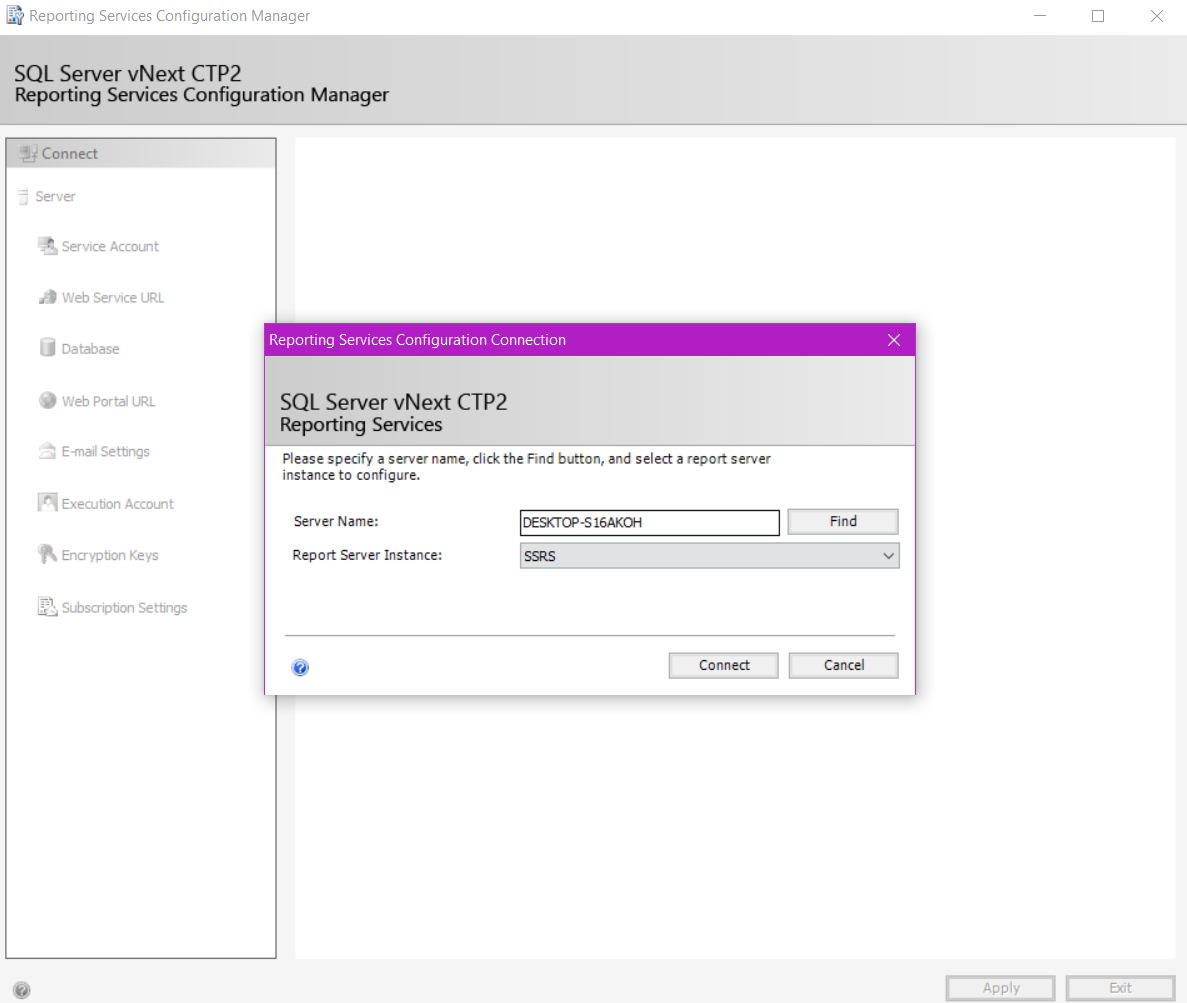
\includegraphics[width=10cm]{./Imagenes/ley1} 
	\end{center}

	\begin{center}
	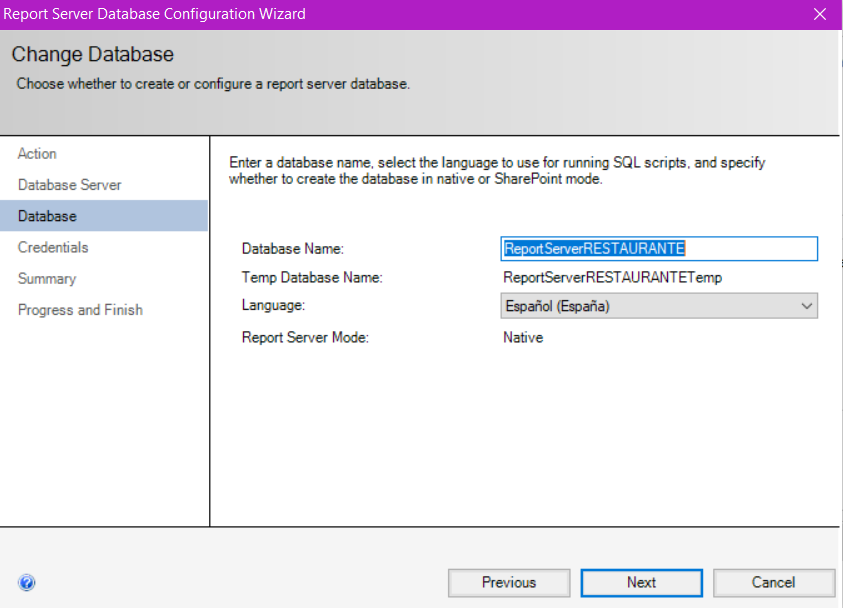
\includegraphics[width=10cm]{./Imagenes/ley2} 
	\end{center}

	\begin{center}
	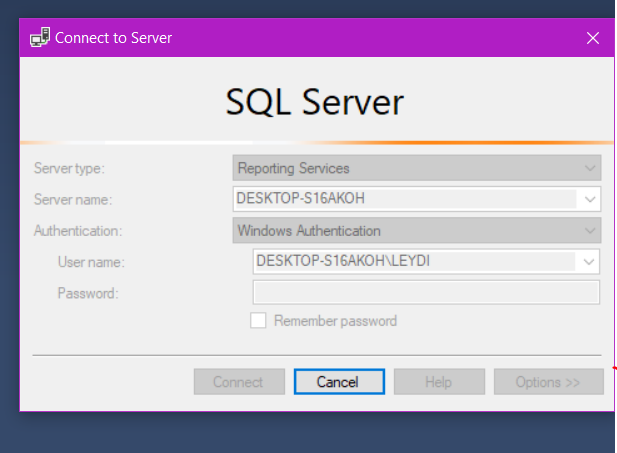
\includegraphics[width=10cm]{./Imagenes/ley3} 
	\end{center}

	\begin{center}
	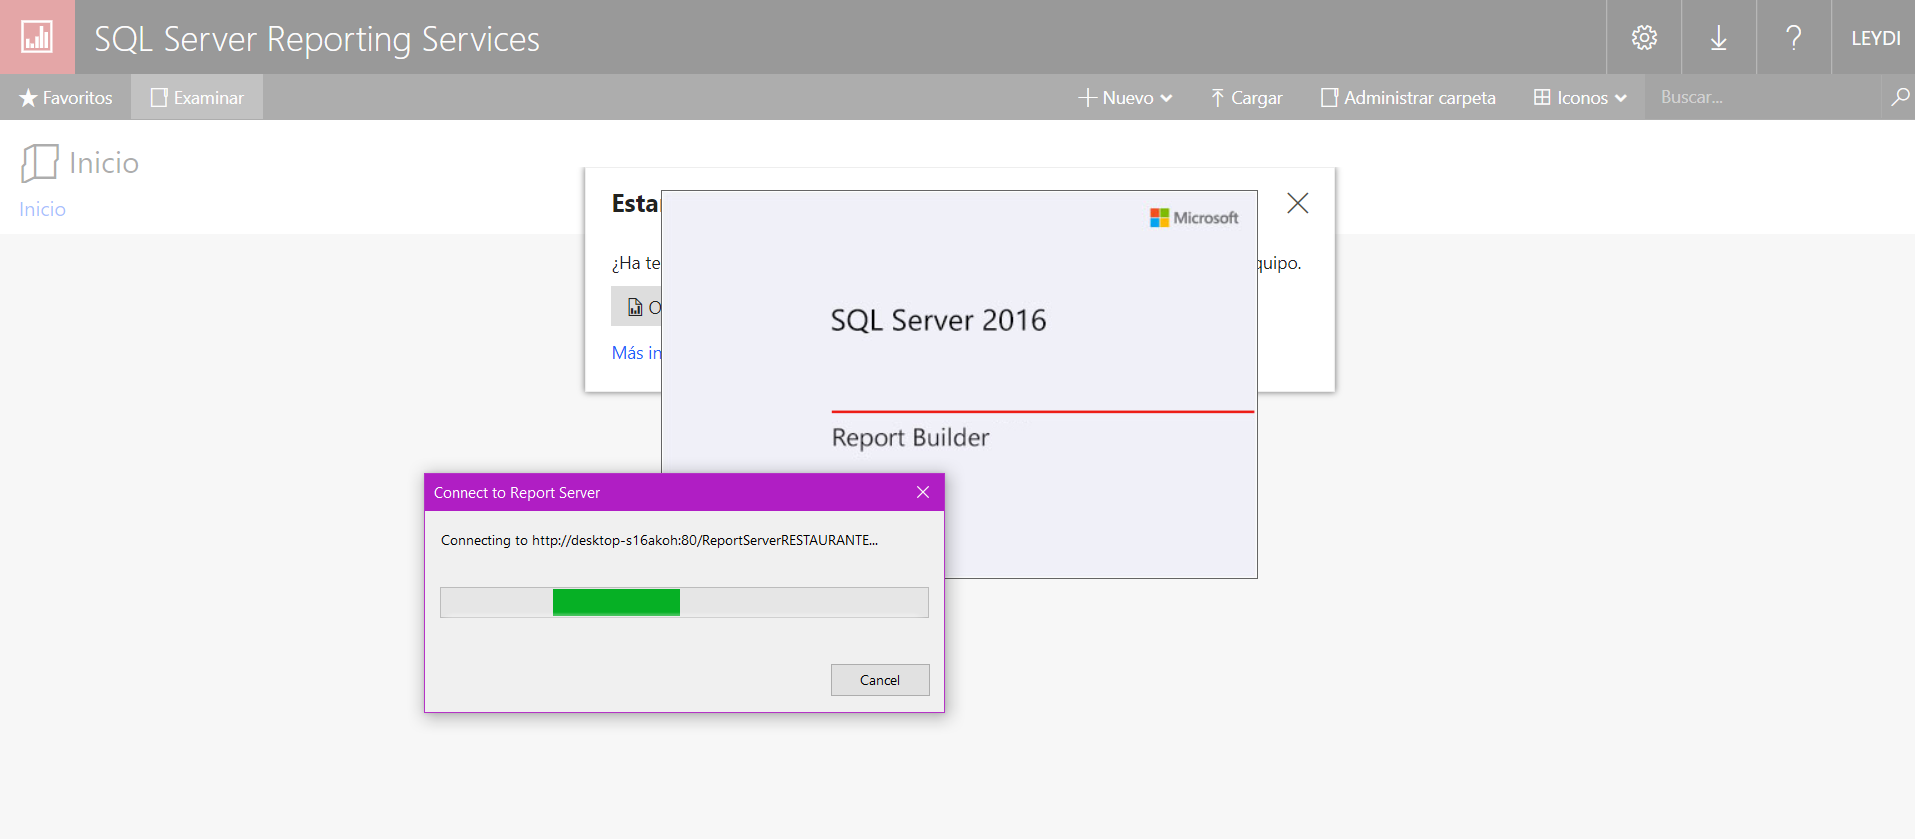
\includegraphics[width=10cm]{./Imagenes/ley4} 
	\end{center}

	\begin{center}
	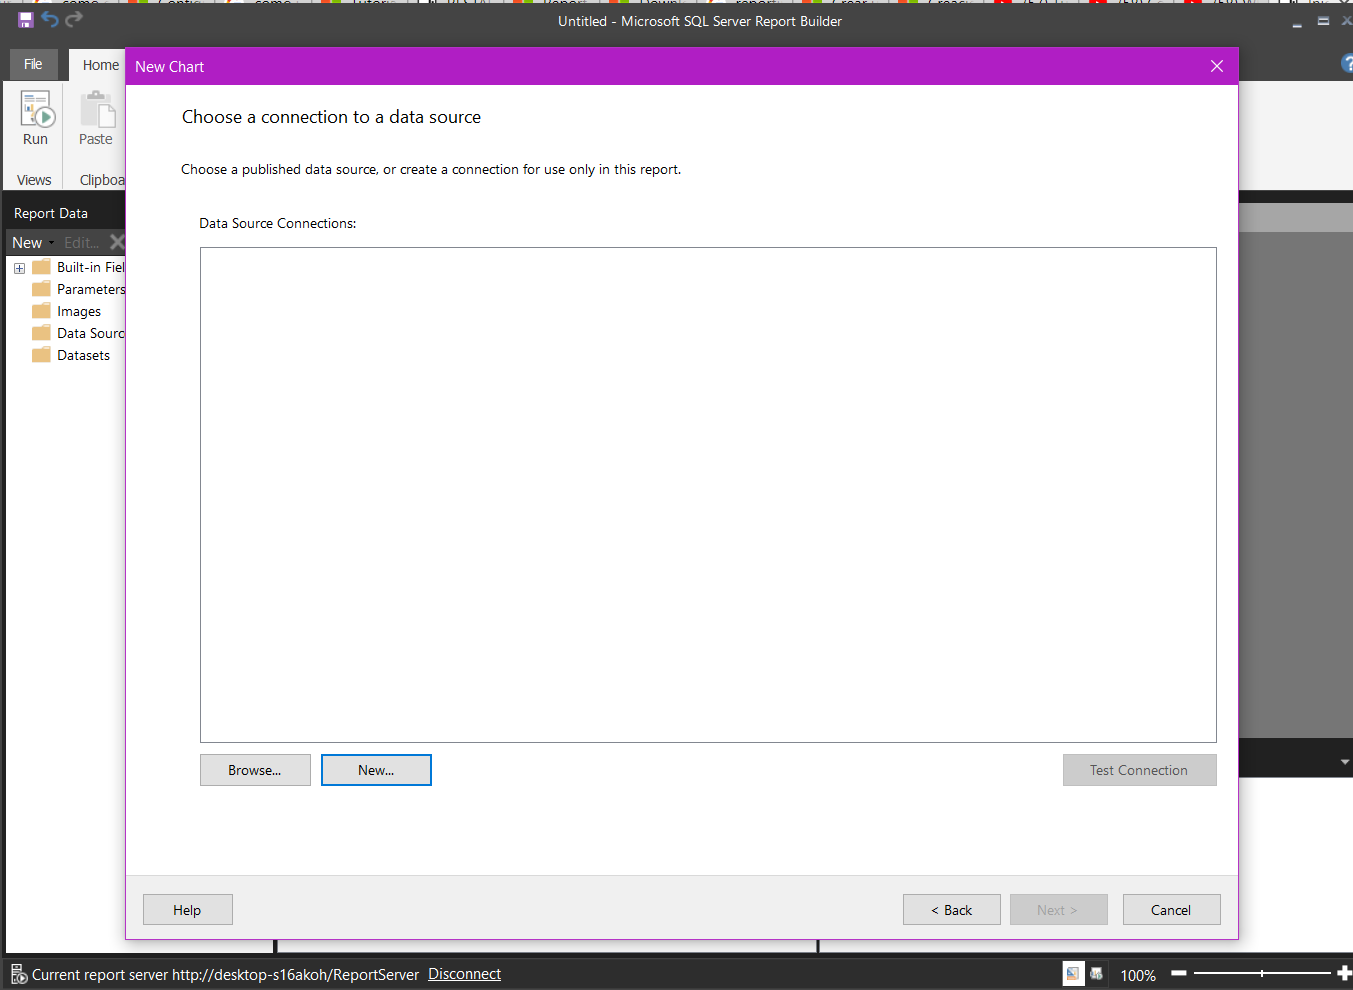
\includegraphics[width=10cm]{./Imagenes/ley6} 
	\end{center}

	\begin{center}
	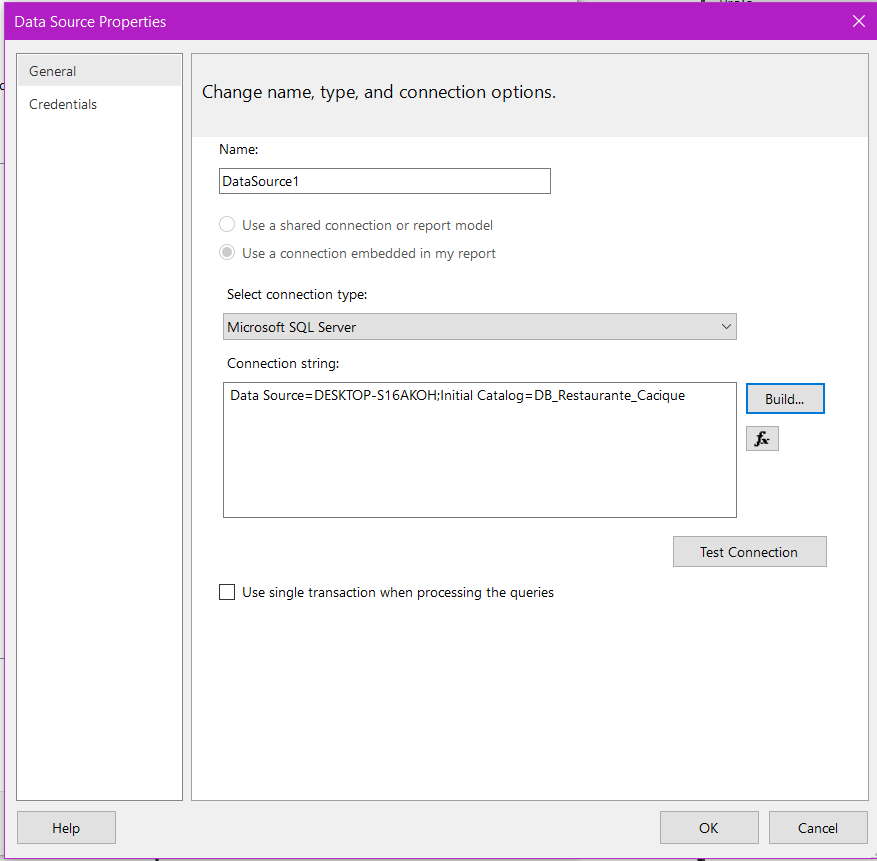
\includegraphics[width=10cm]{./Imagenes/ley7} 
	\end{center}

	\begin{center}
	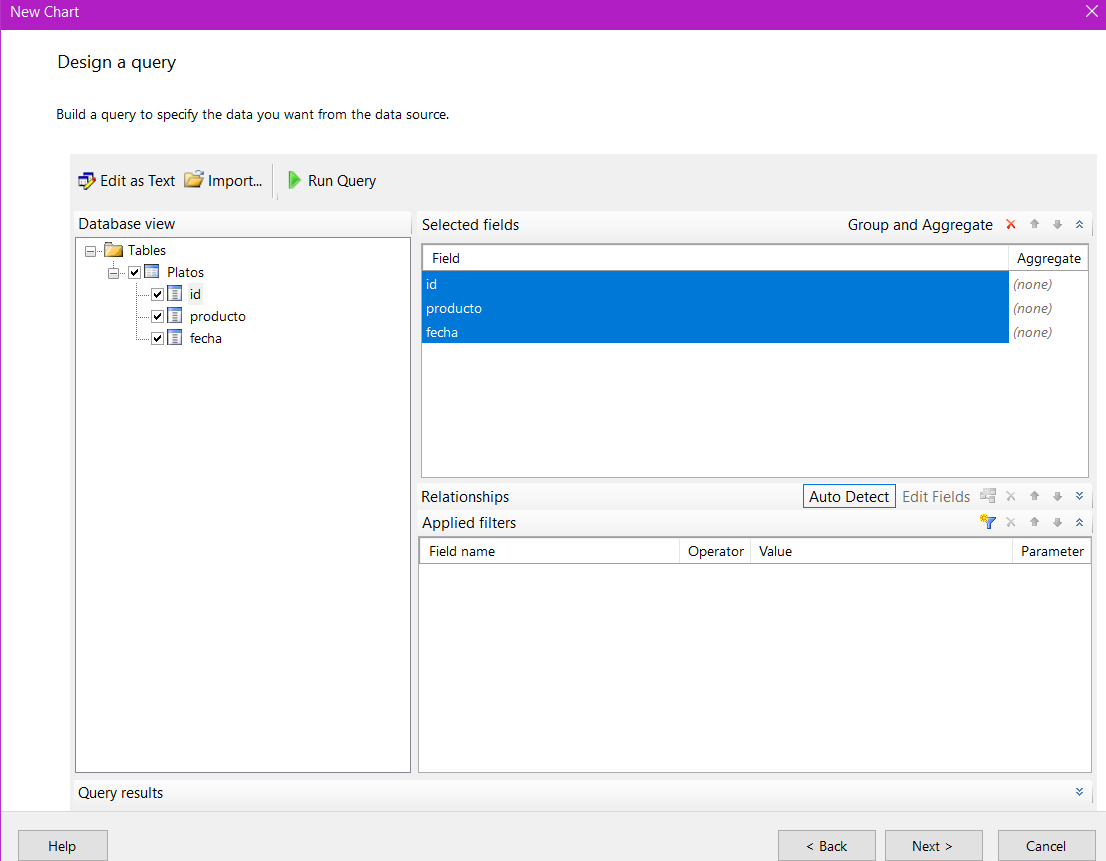
\includegraphics[width=10cm]{./Imagenes/ley8} 
	\end{center}
	
	\begin{center}
	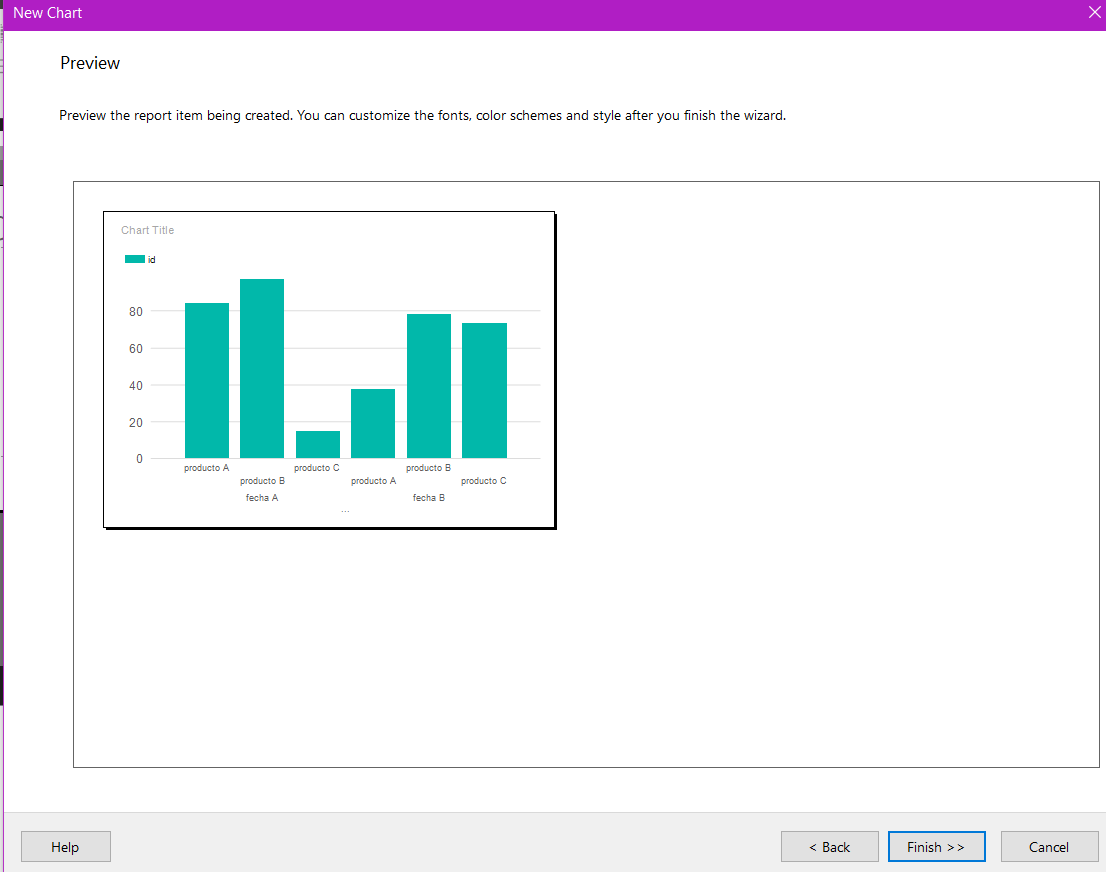
\includegraphics[width=10cm]{./Imagenes/ley9} 
	\end{center}

	\begin{center}
	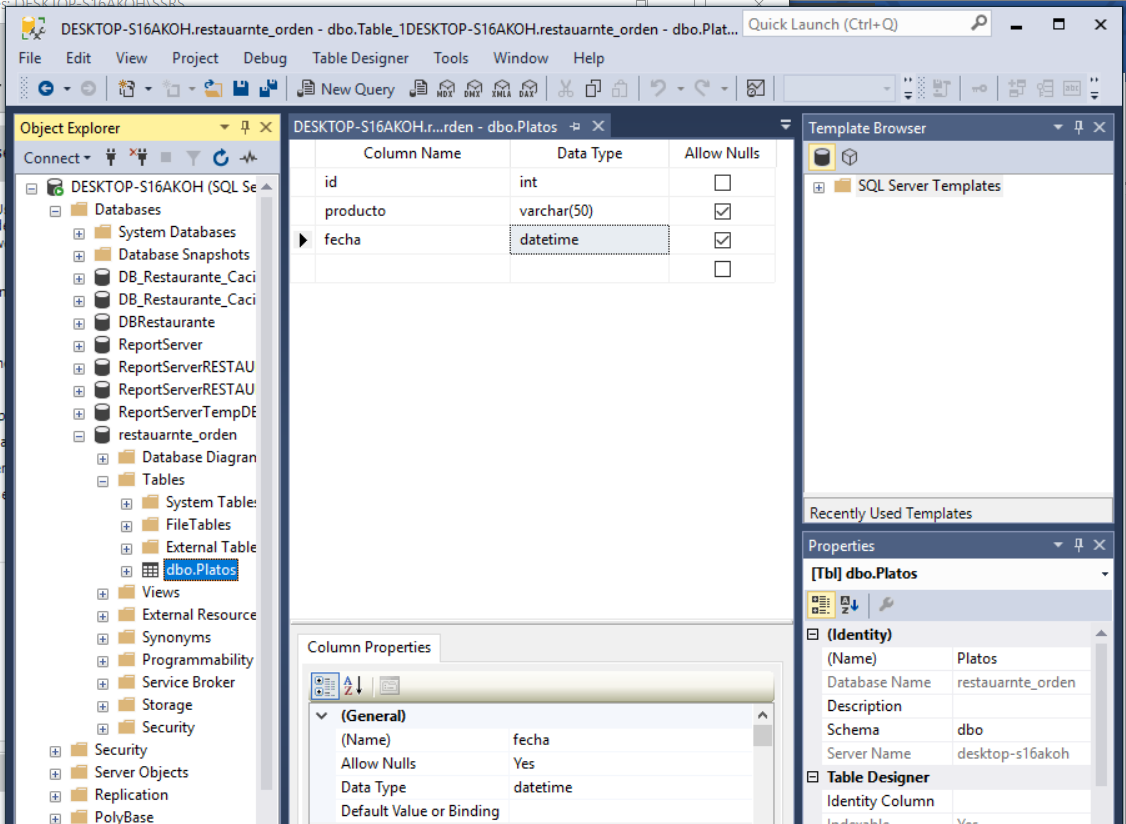
\includegraphics[width=10cm]{./Imagenes/ley10} 
	\end{center}

\section{BALANCED SCORE CARD  } 

\subsection{ DESCRIPCION DEL BALANCED SCORECARD}

	El Balanced Scorecard (BSC) o Cuadro de Mando Integral es un modelo de planificación y gestión que permite alinear a la 			organización con su estrategia. Traduce la estrategia en objetivos relacionados, medidos a través de indicadores y ligados a unos 		planes de acción que permiten alinear el comportamiento de los miembros de la organización.

	Aspectos Claves:
	
	\begin{itemize}
	
		\item  Modelo simple que priorice lo importante
		\item  Utilización de un lenguaje común
		\item  Equipo líder
		\item  Buena comunicación
		\item  Participación de diferentes personas de la organización

	\end{itemize}

	La utilidad del Balanced Scorecard no depende del tipo de empresa, sino de los problemas a los que se enfrenta. El Cuadro de 			Mando Integral se ha implantado en empresas grandes y pequeñas en sectores regulados y no regulados, en organizaciones con 		y sin ánimo de lucro; así como, en empresas con alta rentabilidad y con pérdidas. El cambio depende de nuestro grado de 			satisfacción con el actual modelo de gestión y con la comprensión de la estrategia de la empresa que demuestran las personas de 		nuestra organización.

	A continuación se muestra en un gráfico las fases del Balanced Scorecard.

			\begin{figure}[htb]
				\begin{center}
					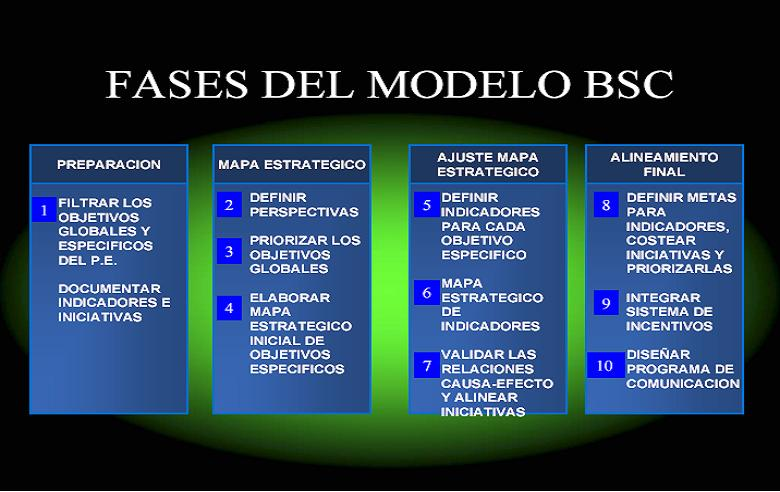
\includegraphics[width=10cm]{./Imagenes/1}
				\end{center}
			\end{figure}

	El Balanced Scorecard no es un reporte de resultados; es un vehículo de comunicación de la estrategia y visión de la compañía. En 		ese sentido, para lograr el éxito en la implementación de la filosofía del BSC se requiere tener el apoyo de los líderes de la 			empresa, quienes deben cumplir los pasos siguientes:

	\begin{itemize}

	\item 	Tener compromiso.
	\item  Crear un modelo de BSC con sus objetivos estratégicos e indicadores clave de desempeño
	\item  Educar al personal, de manera que el BSC sea parte de la cultura organizacional.
	\item  Tener soporte tecnológico (software), en caso no se tenga los recursos necesarios para comprar un software especializado en el tema, se puede utilizar el excel por ser un software muy común en las empresas y contar con herramientas aprovechables en el diseño de formatos para el control del BSC durante la fase de puesta en práctica.
	\end{itemize}

	Es un poderoso instrumento para medir el desempeño corporativo y se ha demostrado que es la herramienta más efectiva para enlazar la visión y la estrategia a cuatro medidas de desempeño, que son:

	\begin{itemize}
		\item Resultados financieros.
		\item Satisfacción de clientes (Internos y externos).
		\item Operación Interna (procesos).
		\item Creatividad, innovación, satisfacción y desarrollo de competencias de los empleados

	\end{itemize}

\subsection{ ELEMENTOS DEL BALANCED SCORECARD}

	Los elementos que conforman el Balanced Scorecard son: el foco estratégico, perspectivas, mapa estratégico, indicadores, metas, iniciativas y responsables de  objetivos o iniciativas.

	\begin{enumerate}[a)]
       	 \item Foco Estratégico o propuesta de valor al cliente
		Selección de aquellos objetivos estratégicos de primer nivel que son prioritarios y que diferenciarán a nuestra organización ante los clientes.

Los focos estratégicos son:

		\begin{itemize}

 		\item[$*$] Liderazgo en Costos: Proporcionar productos y servicios a un precio competitivo para la calidad y funcionalidad que ofrecen.
		\item[$*$] Liderazgo en Producto o Servicios: Se centra en la excelencia de sus productos y servicios, que ofrecen la máxima calidad y funcionalidad.
		\item[$*$] Intimidad con el Cliente: Capacidad de generar vínculos con los clientes para conocerlos y proporcionarles productos y servicios adecuados a sus medidas.

		\end{itemize}

	A continuación se muestra un gráfico en el cual se presenta cada uno de los focos con los temas que estos incluyen.

			\begin{figure}[htb]
				\begin{center}
					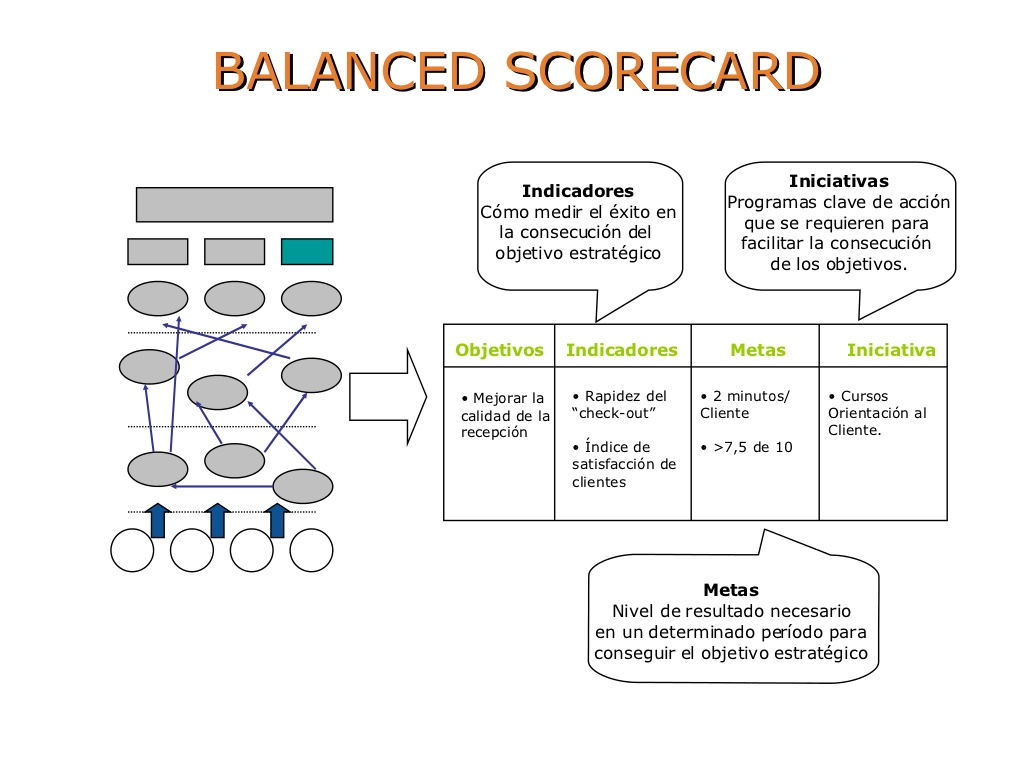
\includegraphics[width=10cm]{./Imagenes/2}
				\end{center}
			\end{figure}


        \item Mapa Estratégico
	Llamamos mapa estratégico al conjunto de objetivos estratégicos que se conectan a través de relaciones causales.
El mapa estratégico ayuda a valorar la importancia de cada objetivo estratégico, ya que nos los presenta agrupados en perspectivas. Las perspectivas son aquellas dimensiones críticas clave en la organización. A continuación, se detallarán las cuatro perspectivas.

		\begin{enumerate}[1.]
   		 \item Perspectiva Financiera

		Las medidas de actuación financiera indican si la estrategia de una empresa, su puesta en práctica y ejecución, están contribuyendo a la mejora del mínimo aceptable. Los objetivos financieros acostumbran a relacionarse con la rentabilidad, medida, por ejemplo, por los ingresos de explotación, los rendimientos del capital empleado, o más recientemente por el valor añadido económico. Otros objetivos financieros pueden ser el rápido crecimiento de las ventas o la generación de cash flow (flujo de caja). Esta definición se puede resumir en la siguiente pregunta: ¿Qué debemos hacer para satisfacer las expectativas de nuestros accionistas?

  		 \item Perspectiva del Cliente

		Identifica los segmentos de clientes y mercado donde se va a competir; así como, mide las propuestas de valor que se orientan a los clientes y mercados. Evalúa las necesidades de los clientes, satisfacción, lealtad, adquisición y rentabilidad; con el fin de alinear los productos y servicios con sus preferencias. Traduce la estrategia y visión en objetivos sobre clientes y segmentos siendo estos los que definen los procesos de marketing, operaciones, logística, productos y servicios.
Entre los principales objetivos que se manejan en esta perspectiva podemos señalar los siguientes: volúmenes de clientes (participación en el mercado y adquisición de nuevos clientes), satisfacción y fidelización de los clientes. Los objetivos de esta perspectiva se pueden resumir en la siguiente pregunta: ¿Qué debemos hacer para satisfacer las necesidades de nuestros clientes?

  		  \item Perspectiva Interna

		Define la cadena de valor de los procesos necesarios para entregar a los clientes soluciones a sus necesidades (innovación, operación y servicio de post venta). Los objetivos e indicadores de esta perspectiva se derivan de estrategias explícitas para satisfacer las expectativas de los clientes.
Se identifican los objetivos e indicadores estratégicos asociados a los procesos clave de la organización o expectativas de clientes y accionistas. Usualmente, esta perspectiva se desarrolla luego que se han definido los objetivos e indicadores de las perspectivas financiera y cliente. Los indicadores de esta perspectiva deben manifestar la naturaleza misma de los procesos propios de la empresa u organización. Los objetivos de esta perspectiva se pueden resumir en la siguiente pregunta: ¿En qué procesos debemos ser excelentes para satisfacer esas necesidades?

		\item Perspectiva de Aprendizaje y Crecimiento

		En esta perspectiva se obtienen los inductores necesarios para lograr resultados en las anteriores perspectivas. La formación y crecimiento de una organización proceden de tres fuentes principales: las personas, los sistemas y los procedimientos de la organización.
La actuación del personal se refuerza con agentes motivadores que estimulen sus intereses hacia la empresa. Se mide en esta perspectiva las capacidades (competencias, creatividad, innovación, entre otros) de los empleados, las capacidades de los sistemas de información, y el clima organizacional para medir la motivación y las iniciativas del personal.


		\end{enumerate}

	 \item Indicadores y Metas

	Los indicadores (también llamados medidas) son el medio que tenemos para visualizar si estamos cumpliendo o no los objetivos estratégicos.
Un objetivo estratégico como por ejemplo el desarrollo de capacidades comerciales del personal clave, puede medirse a través de indicadores. No existen indicadores perfectos, y por eso, para la medición de algunos objetivos estratégicos, se puede utilizar más de uno. Por ejemplo, el desarrollo de esas capacidades comerciales se puede medir a través de indicadores como el número de horas de formación por persona, el índice de satisfacción de los empleados con la formación percibida o el incremento medio de los contratos o ingresos por empleado. Se puede establecer dos tipos de indicadores:

		\begin{itemize}
  		  \item Indicadores de Resultado:Los indicadores de resultado denotan la conclusión de varias acciones tomadas y medidas, la información que dan es definitiva. Mide el éxito en el logro de los objetivos del BSC sobre un período específico de tiempo. Se usan para reportar el desempeño de la organización en la implantación de su estrategia. Para cada indicador como es habitual se debe fijar metas, como regla general debieran ser metas ambiciosas pero posibles de ser logradas.

  		  \item Indicadores de Causa u Operativos: Los indicadores de causa u operativos indican a futuro cual puede ser el resultado de un grupo de acciones u operaciones definidas en un indicador de resultado también se le denomina indicadores inductores de actuación. Provee indicación temprana del progreso hacia el logro de los objetivos; su propósitos es generar los comportamientos adecuados para el logro de la estrategia. Usualmente miden lo que debe “hacerse bien” para alcanzar los objetivos. Miden las palancas de valor, los elementos “impulsores” del desempeño. Su propósito es canalizar y direccionar esfuerzos. También llamados Inductores de Actuación.
  		 
    
 		  \end{itemize}


	 \item Iniciativas Estratégicas
		Las iniciativas estratégicas son las acciones en las que la organización se va a centrar para la consecución de los objetivos estratégicos. Es importante priorizar las iniciativas en función de los objetivos estratégicos. Si analizamos el impacto de las iniciativas en marcha en cada uno de los objetivos estratégicos, podremos visualizar: iniciativas que aportan poco valor al cumplimiento de esos objetivos y objetivos sin soporte en las iniciativas. Las iniciativas pueden tener sus propios indicadores para el seguimiento e incluso un Balanced Scorecard propio.

	\item Responsables y Recursos
		Cada objetivo, indicador e iniciativa debe tener su responsable. Una persona a cargo que controla su cumplimiento.
Otro aspecto clave para una implantación con éxito del Balanced Scorecard es asignar los recursos necesarios para el buen desarrollo de las iniciativas estratégicas. Por ello es necesario establecer los equipos a cargo de cada iniciativa; así como, el papel que diferentes personas van a jugar en ellos. Y también dotar a las iniciativas de los recursos necesarios para su cumplimiento. Se recomienda que el presupuesto contenga una partida de recursos asignados a las iniciativas, estos recursos deben estar diferenciados del presupuesto operativo, del presupuesto de inversiones y otros presupuestos.

    \end{enumerate}


\subsection{ BENEFICIOS DEL BALANCED SCORECARD}

	Los Beneficios de implementar el Balanced Scorecard son:

	\begin{itemize}
   	 \item Comunicar la visión y estrategia a toda la organización.
	\item Traducir objetivos estratégicos y tácticos de la organización en medidas individuales de rendimiento y productividad.
	\item Ofrecer a cada empleado su contribución individual al logro de los objetivos de la empresa.
	\item Ligar los resultados con los procesos que se desarrollaron en el logro de los mismos.
	\item Alinear las estrategias de la empresa con las competencias requeridas del personal.
	\item Monitorear los recursos necesarios para el logro de objetivos.
	\item Elevar los niveles de servicio a clientes internos y externos.

   
  	  \end{itemize}



























\section{DESCRIPCION DE LA EMPRESA} 

Plaza Vea es una cadena de supermercados que forma parte del conglomerado peruano Intercorp, el cual también integra a los supermercados Vivanda.

			\begin{figure}[htb]
				\begin{center}
					
\includegraphics[width=10cm]{./Imagenes/3}
				\end{center}
			\end{figure}

	\begin{itemize}
   	 \item Plaza Vea es la marca de hipermercados y supermercados de la empresa Supermercados Peruanos S.A. perteneciente al prestigioso Grupo Interbank.
	\item	Es una empresa 100 por ciento peruana que da trabajo a más de 10 mil personas en Lima y provincia, distribuidas entre sus más de 80 tiendas, ¡Y seguimos creciendo!
	\item	Fue el primer hipermercado en salir a provincias en el año 2007 lo que nos valió una serie de reconocimientos como el Gran Premio a la Creatividad Empresarial y un Effie de Plata.
	\item	En el 2009 fue elegido como una de las mejores empresas para trabajar en el Perú, ocupamos el puesto 7 en el ranking general de Great Place to work.
	\item	En el 2009 Plaza Vea logra certificación internacional para sus alimentos frescos, es la primera cadena de supermercados del país con certificación HACCP.
	\item	Plaza Vea sigue creciendo por todo el país y se sigue extendiendo.

    
 	 \end{itemize}

MISION:
Somos una empresa peruana de venta de productos al por menor, tanto en perecibles como en abarrotes pasando por textil y electro que basa su desarrollo y crecimiento en una sólida cultura de servicio que busca generar excelentes experiencias de compra para nuestros clientes. Crear excelentes experiencias de compra para que nuestros clientes regresen y tengan una mejor calidad de vida.

VISION:
Ser la primera opción de compra para todos los peruanos siendo Honestos, cuidadosos y ordenado, ser serviciales, muy trabajadores; trabajando en equipo con la búsqueda de un ideal común que nos una con esfuerzo y dedicación, ofreciendo productos de calidad gracias a una capacidad de innovación sostenible en el tiempo. 

\subsection{ ORGANIZACION  DE LA EMPRESA - PLAZA VEA}

Plaza Vea, cuenta con mas 58 locales, logrando de esta manera ser el pilar de la expansión de las operaciones de la empresa tanto en su formato de hipermercado como el de supermercado.

				\begin{figure}[htb]
				\begin{center}
					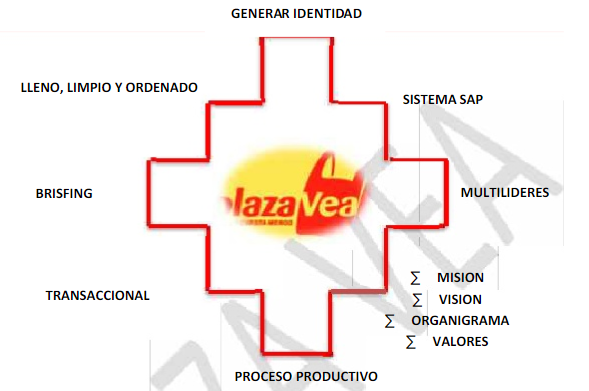
\includegraphics[width=15cm]{./Imagenes/4}
				\end{center}
			\end{figure}



\begin{enumerate}[a)]
        \item Organigrama de la Empresa

			\begin{figure}[htb]
				\begin{center}
					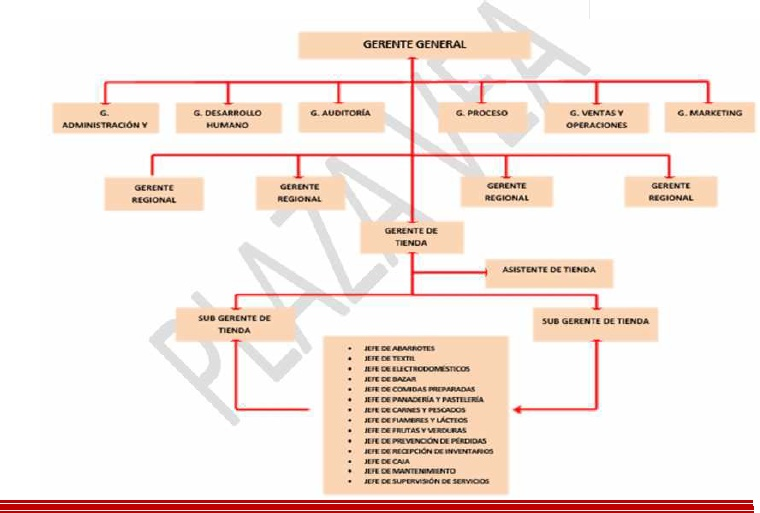
\includegraphics[width=15cm]{./Imagenes/5}
				\end{center}
			\end{figure}
        \item Cadena de Valores

			\begin{figure}[htb]
				\begin{center}
					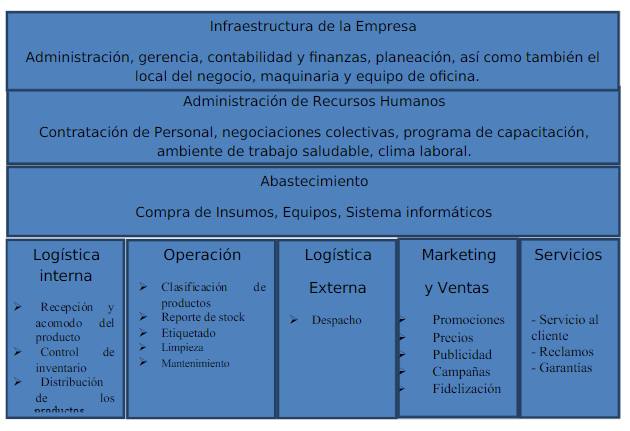
\includegraphics[width=15cm]{./Imagenes/6}
				\end{center}
			\end{figure}

	\item FODA

			\begin{figure}[htb]
				\begin{center}
					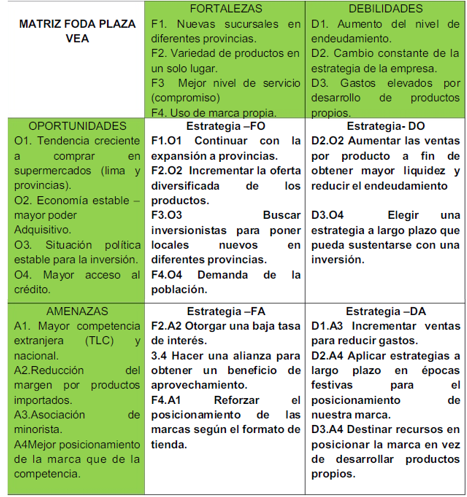
\includegraphics[width=15cm]{./Imagenes/7}
				\end{center}
			\end{figure}

	\item OBJETIVOS ESTRATÉGICOS DE LA EMPRESA PLAZA VEA

		\begin{itemize}
  		  \item[$*$] Capacitar al personal para que este en sintonía con la vocación de servicio y con propósitos de exceder expectativas del cliente.
		\item[$*$] Se la solución diaria y semanal preferida para los consumidores.
		\item[$*$ ]Estar siempre a la Vanguardia; siempre estar en campañas promocionales.
		\item[$*$] Brindar una buena Infraestructura, Comodidad, Seguridad y centros de esparcimiento en nuestras instalaciones.

		\item[$*$] Mantener precios competitivos.
		\item[$*$] Ofrecer un catálogo de productor didácticos en la Web.
		\item[$*$] Promocionar e incentivar la compra electrónica entre ciudadanos peruanos y personas que radican en el extranjero
		\item[$*$] Acaparar nuevos nichos de mercado.
		\item[$*$] Incursionar con más mercados en provincia.
		\item[$*$] Implementación de Data WereHouse
		\item[$*$] Mantener o mejorar la imagen de la empresa.


		\end{itemize}

	\item OBJETIVOS DE ORGANIZACIÓN (APRENDIZAJE E INNOVACIÓN) DE PLAZA VEA

		\begin{enumerate}[1.]
  			  \item Competencias. - dentro de los factores que se han identificado, podemos establecer los
siguientes objetivos:
			\begin{itemize}
  			  \item[$*$] Capacitación para los siguientes factores:

				\begin{itemize}

  				  \item Nivel Profesional adecuado
				  \item Adecuados niveles de productividad
				  \item Baja capacitación en tecnologías de la información
				  \item Personal con poca experiencia técnica
				 \item Bajos niveles de capacitación

				\end{itemize}

			 \item[$*$] Coaching (desarrollo de aptitudes para el liderazgo para mejorar los siguientes aspectos

				\begin{itemize}

  				  \item Alta efectividad en la delegación de funciones
				  \item Alta mayores canales de comunicación

				\end{itemize}

			 \item[$*$] Establecer una relación laboral adecuado para poder tener un manejo adecuado de las relaciones:

				\begin{itemize}

  				  \item Estabilidad laboral
				  \item Limitaciones para atraer gente altamente creativa

				\end{itemize}


			\end{itemize}

  			  \item Clima laboral. - dentro de este aspecto, podemos mencionar los siguientes objetivos:

				\begin{itemize}

				\item[$*$] Crear un clima organizacional adecuado objetivo que busca manejar los efectos del siguiente factor:

				\begin{itemize}

  				  \item Clima organizacional adecuado

				\end{itemize}


				\item[$*$] Cambiar cultura organizacional para manejar adecuadamente los siguientes factores:

				\begin{itemize}

  				  \item Cultura de valores, principios
				  \item Identificación con la empresa

				\end{itemize}


			\end{itemize}
    
		\end{enumerate}

	\item OBJETIVOS INTERNOS DE LA EMPRESA PLAZA VEA

	Los factores que afectan los procesos internos de la empresa han generado los siguientes objetivos:
		\begin{enumerate}[1.]

    		\item Proceso de Innovación. - bajo este proceso se han definido los siguientes objetivos que buscan manejar el efecto de los factores que inciden sobre dichos procesos:

			\begin{itemize}

				\item[$*$] Identificar mercados potenciales, para manejar los factores siguientes:

				\begin{itemize}

  				  \item Empresas interesadas en el sector
				\item Ingreso al Mercado de Lima
				\item Ubicación cercana de mercados potenciales
				\item Adecuadas vías de comunicación
				\item Plan de integración Perú – Ecuador
				\item Sinergia del sistema de Cajas Municipales

				\end{itemize}


				\item[$*$] Crear productos / ofertar nuevos servicios, objetivos que incide sobre los siguientes factores:

				\begin{itemize}

  				  \item Inversión Pública
				\item Privatizaciones
				\item Recuperación del PBI
				\item Condiciones de Libre Mercado
				\item Promoción del Estado a las PYMES
				\item Niveles de desempleo y subempleo
				\item Promoción del Banco Agropecuario
				\item Normas tributarias del sector 


				\end{itemize}

			\end{itemize}

   		\item Procesos de Operaciones. - los procesos de operaciones se establecen con la finalidad de
buscar la eficiencia en lo que hacemos para brindar nuestros productos. Dentro de estos
procesos se han definido los siguientes objetivos:


			\begin{itemize}

				\item[$*$] Mejorar niveles de productividad

				\begin{itemize}

  				  \item Nivel adecuado de tecnificación interna
				\item Desarrollo tecnológico mundial
				\item Intercambio técnico por la globalización
				\item Desarrollo tecnológico de la competencia
				\item Orientación empresarial


				\end{itemize}


				\item[$*$] Minimizar el efecto de factores políticos.

				\begin{itemize}

  				  \item Débil estabilidad jurídica
				\item Débil estabilidad política
				\item Injerencia política
				\item Normas de austeridad y contratación del Estado


				\end{itemize}
				\end{itemize}


   		\item Procesos de comercialización.- Para manejar un valor más adecuado de los productos o
servicios que ofrecemos, se definen los siguientes objetivos: 

				\begin{itemize}

				\item[$*$] Incrementar participación de mercado

				\begin{itemize}

  				  \item Participación de mercado
				\item Retiro de bancos comerciales de provincias
				\item Poco acceso a organismos privados y públicos
				\item Zona geográfica con clima inestable

				\end{itemize}

				\end{itemize}


    
		\end{enumerate}

	\item OBJETIVOS DEL CLIENTE DE LA EMPRESA PLAZA VEA

		\begin{itemize}

				\item[$*$] Atributos.- dentro de este concepto podemos establecer los siguientes objetivos estratégicos:

				\begin{itemize}

  				  \item Mantener Precios Competitivos
				\item Tasas de interés competitivas
				\item Mejorar constantemente la Calidad del Producto
				\item Producto exclusivo y de calidad
				\item Diversificar los productos que ofrece la CMAC
				\item Falta mayor diversificación de productos


				\end{itemize}


				\item[$*$] Imagen.- los objetivos definidos para el caso del atributo de imagen dentro de la perspectiva de cliente son los siguientes:
				\begin{itemize}

  				  \item Proyectar imagen de solidez y confianza
				\item Limitada infraestructura

				\end{itemize}

				\item[$*$] Relaciones con el cliente.- Se han establecido los siguientes objetivos:

				\begin{itemize}

  				  \item Establecer un Programa de CRM (Customer Relationship Management)
				\item Lealtad y satisfacción del cliente
				\item Promoción y formalización de negocios
				\item Falta programa de administración de clientes

				\end{itemize}

		\end{itemize}

	\item OBJETIVOS FINANCIEROS DE LA EMPRESA PLAZA VEA
		
	Dentro de la perspectiva financiera tenemos los siguientes objetivos:

			\begin{itemize}

  				  \item Incrementar el valor patrimonial, dentro de este objetivo se enmarcan los siguientes factores:
				\item Crecimiento sostenido
				\item Rentabilidad adecuada
				\item Capacidad de Endeudamiento
				\item Reducir costos operativos, este objetivo busca manejar los siguientes factores:
				\item Limitados fondos internos
				\item No existe metodología de costeo eficaz
				\item Diversifica fuentes de financiamiento, para manejar una adecuada estructura financiera:
				\item Líneas de financiamiento externas para microfinanzas
				\item Reducir efecto de factores externos, para minimizar los efectos de:
				\item Nivel de la inflación
				\item Incremento de la devaluación
				\item Percepción de riesgo país


			\end{itemize}

	\item MAPA ESTRATEGICO DE LA EMPRESA PLAZA VEA


	Para el Desarrollo del Mapa Estratégico y Balanced ScoreCard de la Empresa Plaza Vea, se utilizó el software de Reportes Tableau.
Tableau es un software de análisis de datos con una excelente capa de visualización y presentación, considerado por muchos como uno de los mejores programas para la presentación visual de datos y con muy alta clasificación en la facilidad de uso, por lo que sigue muy de cerca a Microsoft Excel.

			\begin{figure}[htb]
				\begin{center}
					
\includegraphics[width=10cm]{./Imagenes/8}
				\end{center}
			\end{figure}


			\begin{figure}[htb]
				\begin{center}
					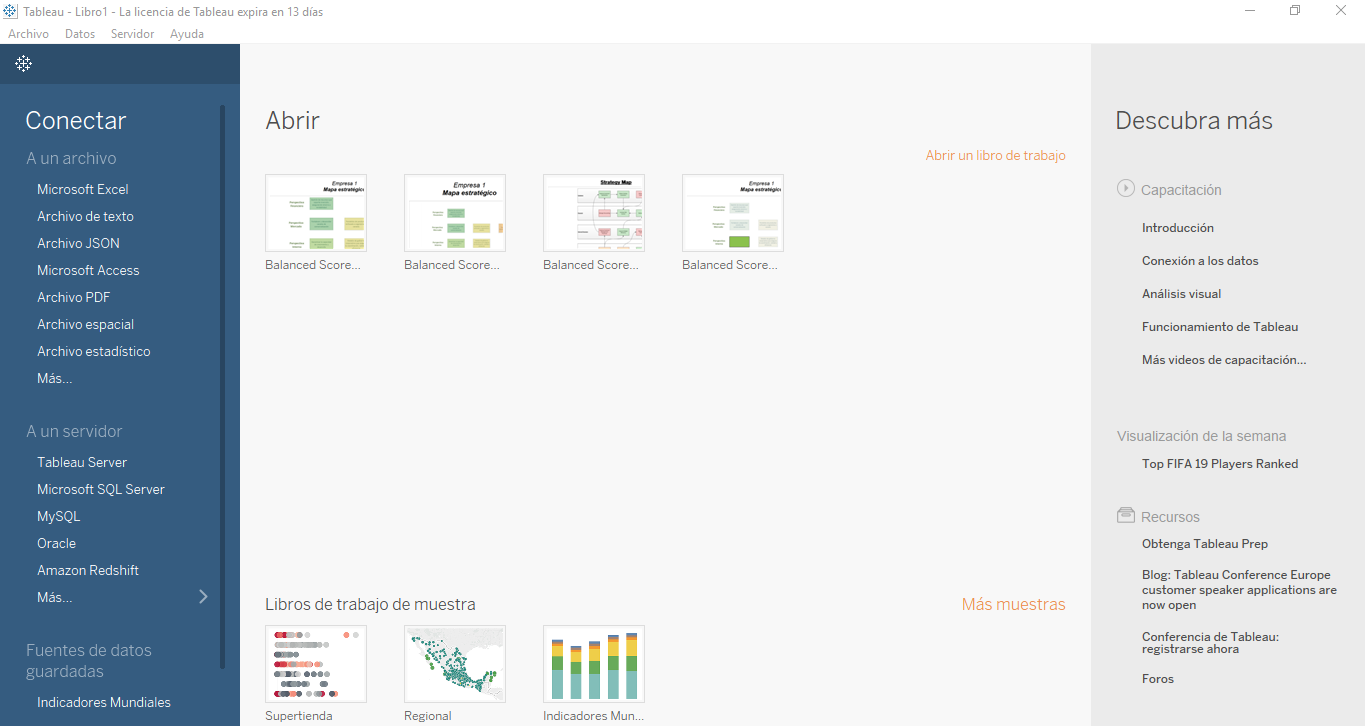
\includegraphics[width=17cm]{./Imagenes/9}
				\end{center}
			\end{figure}


			\begin{figure}[htb]
				\begin{center}
					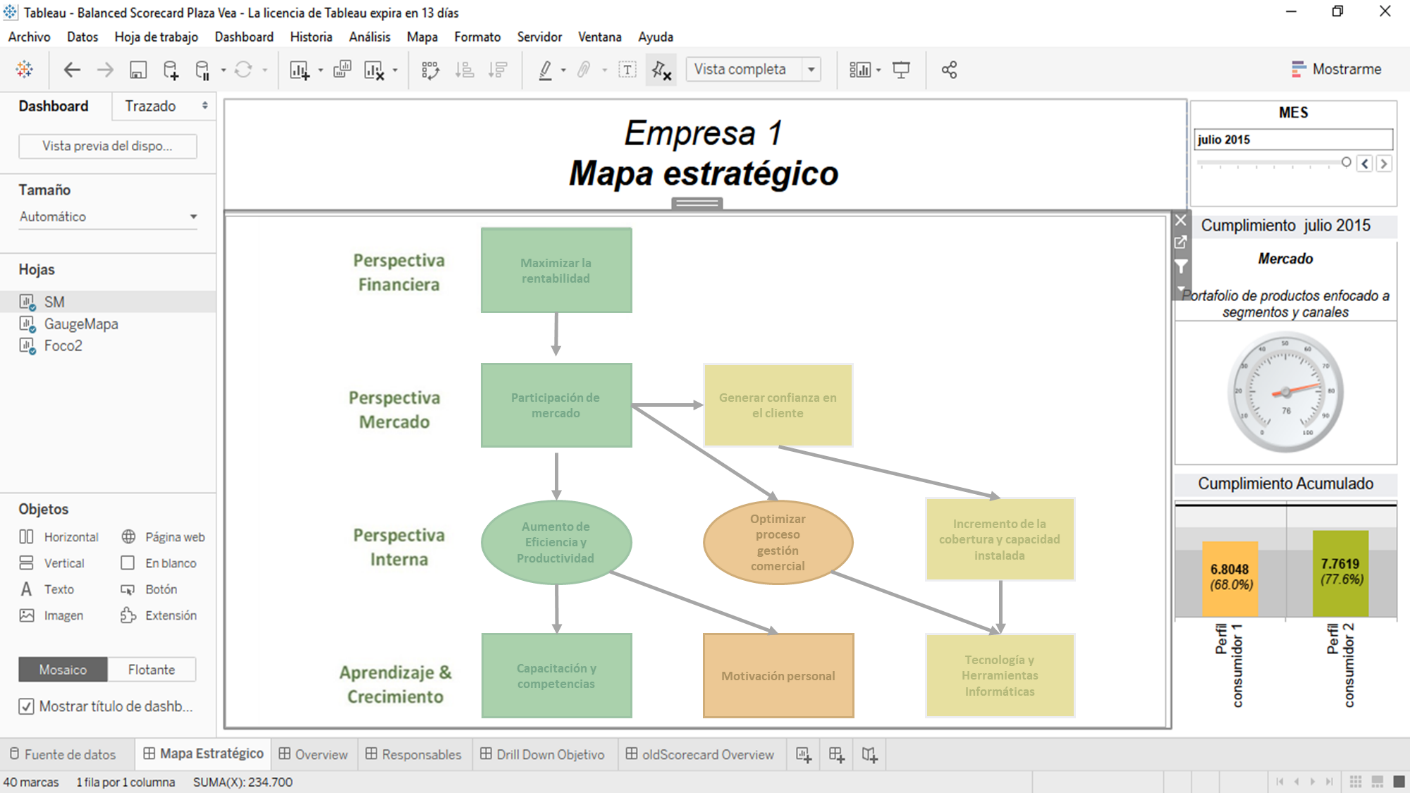
\includegraphics[width=17cm]{./Imagenes/10}
				\end{center}
			\end{figure}


			\begin{figure}[htb]
				\begin{center}
					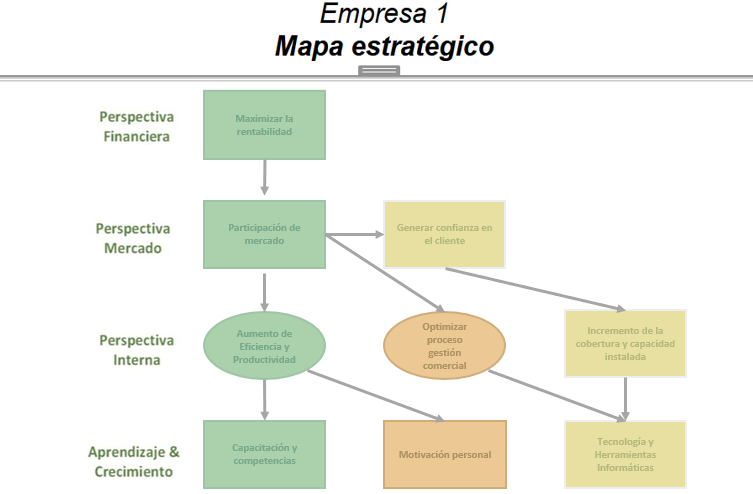
\includegraphics[width=17cm]{./Imagenes/11}
				\end{center}
			\end{figure}

	\item BALANCED SCORECARD DE LA EMPRESA PLAZA VEA

			\begin{figure}[htb]
				\begin{center}
					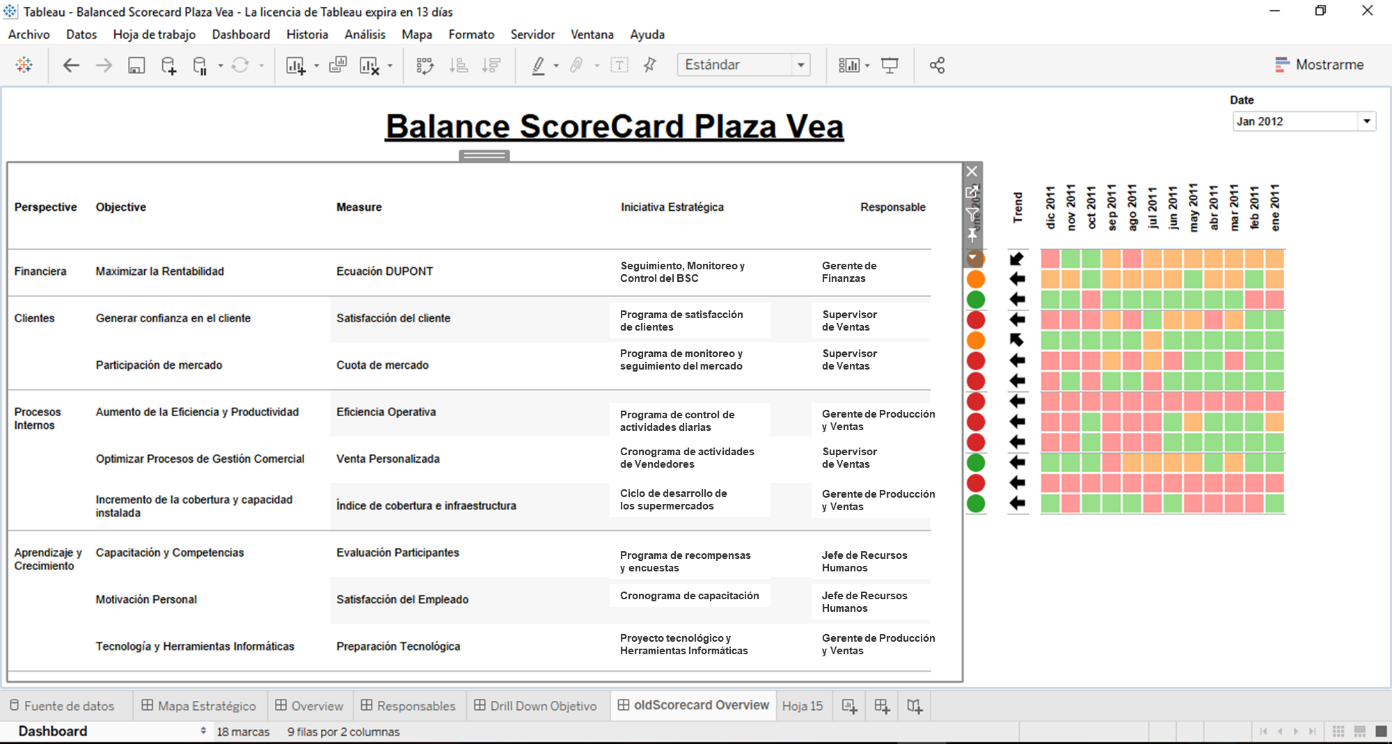
\includegraphics[width=17cm]{./Imagenes/12}
				\end{center}
			\end{figure}

			\begin{figure}[htb]
				\begin{center}
					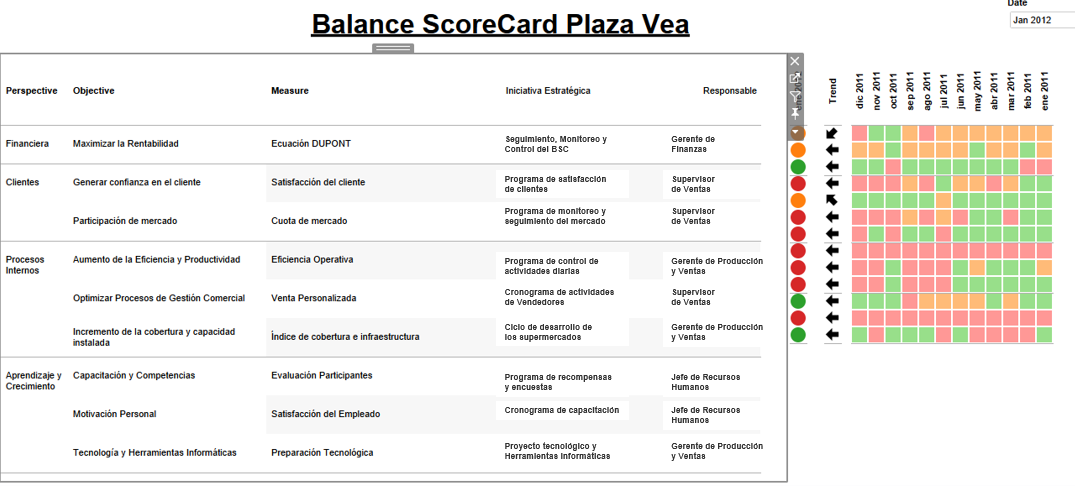
\includegraphics[width=17cm]{./Imagenes/13}
				\end{center}
			\end{figure}

    \end{enumerate}
	
	

\end{document}
